\documentclass[conference]{IEEEtran}
\IEEEoverridecommandlockouts
% The preceding line is only needed to identify funding in the first footnote. If that is unneeded, please comment it out.
\usepackage{cite}
\usepackage{amsmath,amssymb,amsfonts}
\usepackage{algorithmic}
\usepackage{graphicx}
\usepackage{textcomp}
\usepackage{xcolor}
\def\BibTeX{{\rm B\kern-.05em{\sc i\kern-.025em b}\kern-.08em
    T\kern-.1667em\lower.7ex\hbox{E}\kern-.125emX}}
\begin{document}

\title{Learning and Enhancement of Visual Place Recognition Methods\\
{\footnotesize \textsuperscript{*}Note: This is for AER 1515 course project.}
\thanks{
% Identify applicable funding agency here. If none, delete this.
}
}

\author{\IEEEauthorblockN{Zhenyuan Xiang}
\IEEEauthorblockA{\textit{ Department of Electrical \& Computer Engineering } \\
\textit{University of Toronto}\\
Toronto, Canada \\
zhenyuan.xiang@mail.utoronto.ca}
\and
\IEEEauthorblockN{ Zhentao Fan}
\IEEEauthorblockA{\textit{ Department of Electrical \& Computer Engineering } \\
\textit{University of Toronto}\\
Toronto, Canada \\
zhentao.fan@mail.utoronto.ca}
% \and
% \IEEEauthorblockN{3\textsuperscript{rd} Given Name Surname}
% \IEEEauthorblockA{\textit{dept. name of organization (of Aff.)} \\
% \textit{name of organization (of Aff.)}\\
% City, Country \\
% email address or ORCID}
% \and
% \IEEEauthorblockN{4\textsuperscript{th} Given Name Surname}
% \IEEEauthorblockA{\textit{dept. name of organization (of Aff.)} \\
% \textit{name of organization (of Aff.)}\\
% City, Country \\
% email address or ORCID}
% \and
% \IEEEauthorblockN{5\textsuperscript{th} Given Name Surname}
% \IEEEauthorblockA{\textit{dept. name of organization (of Aff.)} \\
% \textit{name of organization (of Aff.)}\\
% City, Country \\
% email address or ORCID}
% \and
% \IEEEauthorblockN{6\textsuperscript{th} Given Name Surname}
% \IEEEauthorblockA{\textit{dept. name of organization (of Aff.)} \\
% \textit{name of organization (of Aff.)}\\
% City, Country \\
% email address or ORCID}
}

\maketitle

\begin{abstract}
This course project is an implementation for the Visual Place Recognition(VPR) problem. The ground method that is being used is Bag of Visual Words(BoVW). We tried different ways to accelerate the runtime and to improve the accuracy of the algorithm by integrating it with Region of Non-Interest (RoNI) detection and Landmark detection.\\
\end{abstract}

\begin{IEEEkeywords}
Visual Place recognition, Bag of Visual Words, YOLO, Region of Non-Interest
\end{IEEEkeywords}

\section{Introduction}

Visual Place Recognition (VPR) is an important part of computer vision technology. It's used to help computers and robots figure out where they are by looking at images of different places. This has strong implications in various cutting-edge applications like autonomous driving, robotic navigation, and augmented reality. Variability in lighting, seasonal changes, and different viewpoints can drastically alter the appearance of a location in images, which raises the difficulties of this problem.

The Bag of Visual Words (BoVW) model, inspired by the Bag of Words concept in text analysis, is a notable approach to tackling the VPR challenge. This method involves extracting key features from images and representing them as a collection of "visual words," thereby transforming complex visual inputs into a simplified, yet effective, format for analysis. While BoVW has shown promising results in VPR, its performance can be impacted by the same environmental factors that challenge VPR as a whole.

Now, with new advancements in learning from data, especially deep learning, we can try to make BoVW even better. This course project is about doing just that. We're investigating adding two new parts to the BoVW method: Region of Non-Interest (RoNI) detection and Landmark/feature object detection. RoNI detection helps the computer ignore parts of the image that aren't useful for figuring out where it is, like moving cars or people. Landmark detection, on the other hand, is about finding special features in the environment that are easy to recognize and don't change much, which can help the computer figure out its location more accurately.

This paper talks about how we used these new ideas to see if they improve BoVW for VPR. We're hoping that by adding these parts, we can help computers and robots understand where they are more quickly and accurately.


\textbf{[discussion of related work required]}

\section{Problem Definition}

\subsection{Input}

An image of a target spot that is captured by a camera either from human beings or robots.

\subsection{Output}

A label or a name of the spot that the photo/image is taken from.

\subsection{Domain \& Range}

Since the model is trained with offline data for now, the output is limited to the places that we have collected and labeled in our dataset. The input can be any image, but only the image taken from the location that has been collected and labeled would get a reasonable prediction/result.

\section{Methods and Algorithms}

As mentioned earlier, we are using BoVW as our ground model and we are investigating two possible optimizations of RoNI detection and Landmark detection.

\subsection{Bag of Visual Words}

We first implement a primitive BoVW and here are the stages and steps for a native BoVW method. \\

\textbf{Stage 1.} Loading Images from the training set

Step 1: The process begins with loading a collection of images. These images form the training set and are used to build the visual vocabulary. Each image in this set represents a different location and contains various features that can be used for place recognition. The dataset we have used includes the spots that we collected in St. George campus at University of Toronto as well as GSV-Cities dataset. \textbf{ \{ reference missing \} }
\\

\textbf{Stage 2.} Feature Detection and Description

Step 2: Using an OpenCV feature detector SIFT (Scale-Invariant Feature Transform), keypoints in each image are detected. Keypoints are distinctive points in the image that are easily recognizable regardless of scaling or rotation (like edges, corners, or blobs).

Step 3: For each keypoint detected, a descriptor is calculated. This descriptor is a vector of numbers that represents the keypoint's characteristics, such as its texture, intensity, orientation, etc. These descriptors are crucial for identifying and matching similar features across different images.\\

\textbf{Stage 3.} Building the Visual Vocabulary

Step 4: The descriptors from all images in the training set are then used to build a visual vocabulary. This is achieved through a clustering algorithm, which k-means in our case. The descriptors are grouped into clusters, with each cluster representing a 'visual word'. The idea is to categorize similar features together, forming a dictionary of visual words.\\

\textbf{Stage 4.} Quantization of Features and Histogram Building

Step 5: Once the visual vocabulary is established, each descriptor in new images is matched to the closest visual word in the vocabulary. 

Step 6: For each image, a histogram is then created based on how frequently each visual word occurs. This histogram effectively converts the image into a fixed-size vector, where each dimension represents a visual word, and the value in that dimension is the frequency of the word in the image.\\

\textbf{Stage 5.} Training the Support Vector Machine (SVM)

Step 7: The final step involves using these histograms to train a machine learning model. In this case, a linear Support Vector Machine (SVM) is used. The SVM is trained with histograms from the training images, along with their corresponding location labels. 

Step 8: The trained SVM model can then classify or predict the location label of a new image based on its histogram. The SVM works by finding the best boundary that separates the histograms of images from different locations.

\subsection{RoNI}

Based on the primitive BoVW implementation, we found the algorithm performs poorly when there is a large proportion of the testing image is green vegetation. So one direct attempt is to reduce the reliance on the descriptors for features of green vegetation. Also, intuitively, as the objects like vehicles are moving now and then, descriptors for those variant object should not be heavily used for our locations classification problem. 

Therefore, we are implementing RoNI to see if it works.

\textbf{ \{ example for leaf image missing \} }

\textbf{ \{ actuall data analysis missing \} }

\paragraph{Overview}

Region of Non-Interest (RoNI) is a method that can enhance the effectiveness of our Visual Place Recognition (VPR) system. In our project, the RoNI method is designed to identify and mask out transient or variant objects such as people, cars, and other movable objects, which typically do not contribute to the reliable recognition of a place.

\paragraph{Object Detection with YOLO}

The RoNI method employs YOLO (You Only Look Once), a state-of-the-art deep learning object detection system. YOLO is known for its speed and accuracy in detecting objects in real-time.

YOLO scans the entire image and identifies objects that fall into predefined categories, such as people, vehicles, and other transient objects. Specifically, for our project, we mask out types of objects listed in 
\begin{verbatim}
    EXCLUDE_NAMES = set([
        'person',
        'bicycle',
        'motorbike',
        'car',
        'bus',
        'truck',
    ])
\end{verbatim}

Each detected object is localized and bounded by a rectangle (bounding box).
Creating a Non-Interest Mask:

Based on the object detections, a mask is created for each image. This mask covers all identified transient objects. Essentially, areas within the bounding boxes are marked as regions of non-interest.

The masking process ensures that these transient or variant features do not influence the feature extraction process, focusing the attention of the VPR system on stable and permanent environmental features.

\paragraph{Integration with Feature Extraction}

In the feature extraction phase, typically involving SIFT, the RoNI mask is applied. This means that features within the masked regions are not processed or considered in the subsequent steps.

By applying the RoNI mask, we ensure that our feature set primarily consists of stable and distinct environmental characteristics, which are more reliable for place recognition.

\paragraph{VPR Accuracy and the Experiments}

The exclusion of transient features like cars and pedestrians, which may not be present consistently in every image of the same location, actually decreases 1\% to 2\% of the accuracy of place recognition. This is not what we expected. This experiment just tells us that those features can somehow benefit our model and are informative in the end. Removing them directly would lead to a loss of some critical information that is required for identifying a location.

\textbf{ \{ further explaination \} }
\textbf{ \{ algo for removing vegetation \} }

\\

\subsection{Landmark Detection}
\begin{figure}[htbp]
\centerline{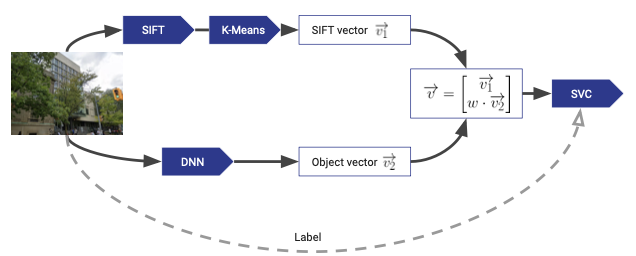
\includegraphics[width=9cm]{landmark.png}}
\caption{Landmark Detection Algorithm.}
\label{fig}
\end{figure}
\paragraph{Overview}
Our project has incorporated an enhanced landmark detection feature into the Bag of Visual Words (BoVW) method to further improve the accuracy of Visual Place Recognition (VPR). This improvement focuses on detecting specific feature objects in the environment, which act as unique identifiers or landmarks.

Implementation and Features:

\paragraph{Landmark Detection Using Pretrained YOLOv5}

Still, we utilized the pre-trained YOLOv5 model for object detection. YOLO's ability to quickly identify specific objects in images makes it ideal for enhancing our VPR system with landmark detection capabilities.

\paragraph{List of Feature Objects}

The feature objects targeted by our system include:

\begin{verbatim}
    INTERESTING_OBJ_LIST = [
        'traffic light',
        'fire hydrant',
        'stop sign',
        'parking meter',
        'bench'
    ]
\end{verbatim}

These objects were selected because they are commonly found in urban environments and are relatively static and distinctive, making them excellent landmarks for place recognition.

\paragraph{Integration with BoVW}

In our modified BoVW approach, each detected landmark object is treated as a separate 'word'. This means that these objects contribute uniquely to the visual vocabulary used in place recognition.

To emphasize the importance of these landmarks, we weight the frequency vector of the feature objects and stack it with the original frequency vector from BoVW. This weighting gives more prominence to landmarks in the final image representation.

\paragraph{Optimization of Weighting Factor}

Through experimentation, we determined that the optimal weighting factor for these feature objects is 10. This value was found to provide the best balance between emphasizing landmarks and maintaining the overall integrity of the feature set.

\textbf{ \{ add pictures for illustration \} }

\paragraph{Performance and Results}

% \begin{figure}[htbp]
% \centerline{\includegraphics{comparison for landmark.png}}
% \caption{Example of a figure caption.}
% \label{fig}
% \end{figure}
% \textbf{ \{ add charts here\} }
\begin{table}[h]
\centering
\caption{Landmark Detection Result}
\label{my-label}
\begin{tabular}{|c|c|c|c|}
\hline
$\#$ of places &  Accuracy($\%$)  &  Train Time($\%$)   &  Test Time($\%$)   \\ \hline
50 & 80.24\% & 66.61 & 6.91 \\ \hline
100 & 76.98\% & 127.23 & 9.06 \\ \hline
200 & 72.55\% & 246.73 & 13.88 \\ \hline
\end{tabular}
\end{table}

\begin{table}[h]
\centering
\caption{Comparison with the previous result}
\label{my-label}
\begin{tabular}{|c|c|c|c|}
\hline
$\#$ of places & $\Delta$Accuracy($\%$)  & $\Delta$Train Time($\%$)   & $\Delta$Test Time($\%$)   \\ \hline
50 & 1.32\% & 19.06 & 79.87 \\ \hline
100 & 1.28\% & 17.75 & 74.06 \\ \hline
200 & 1.66\% & 17.08 & 64.58 \\ \hline
\end{tabular}
\end{table}

When compared to our previous results without landmark detection, there was a noticeable increase in accuracy. Specifically, the accuracy increased by 1.32\% for 50 places, 1.28\% for 100 places, and 1.66\% for 200 places.

Importantly, this improvement in accuracy was achieved without a proportional increase in training or testing time. In fact, the percentage increase in training and testing times was considerably lower than the improvement in accuracy, making this a highly efficient enhancement.

\paragraph{Future Potential}


Currently, our system only considers five types of objects as landmarks. Expanding this list to include more diverse and location-specific objects could further improve accuracy.
For instance, incorporating the detection of unique building styles or other permanent urban features could provide more distinctive cues for place recognition.

Further refinement and customization of the landmark detection algorithm could optimize its performance specific to the environments and datasets being used.
In conclusion, the integration of landmark detection into our VPR system represents a significant advancement, enhancing the accuracy and robustness of place recognition. The success of this approach suggests great potential for future improvements and expansions in this direction.


\\

\section{Dataset}

\paragraph{Overview}
Our project utilizes the GSV-Cities dataset\textbf{ \{ reference missing \} }, which is specifically designed for tasks in Visual Place Recognition (VPR). This dataset is extensive, containing around 530,000 images from over 62,000 different locations. The variety of images, each taken from multiple angles and under various lighting and time conditions, makes it an ideal choice for VPR research.

It encompasses approximately 530,000 images, encompassing a diverse array of over 62,000 distinct locations. This extensive range offers a robust foundation for training and testing VPR algorithms.

\paragraph{Characteristics of the Dataset}
The images in the GSV-Cities dataset are rich in diversity, with each location represented by 4 to 20 different images. This diversity is crucial as it simulates the real-world scenarios where conditions change constantly. Furthermore, every image in this dataset is accurately labeled with essential information like the city name, place ID, and the date (year and month) it was captured, providing a reliable ground truth for our experiments.

\paragraph{Data Selection and Randomization}
To optimize the dataset for our specific research needs, we employed custom scripts \textbf{ \{ details missing \} } to select and randomize the data. This process ensures that the training and testing sets are comprehensive and unbiased, reflecting the diversity inherent in the dataset. Randomization is key to avoiding biases in our experiment and ensuring that our findings are applicable to various real-world situations.

\paragraph{Dataset’s Role in the Project}
The GSV-Cities dataset forms the backbone of our training and testing phases, allowing us to thoroughly evaluate the performance of the enhanced BoVW method. Given its diverse nature and detailed labeling, the dataset provides an excellent benchmark for assessing the effectiveness of the improvements we have integrated, such as RoNI detection and Landmark detection.



\section{The Deliverable}


\textbf{ \{ The following is not the part of this paper \} }

\\

Before you begin to format your paper, first write and save the content as a 
separate text file. Complete all content and organizational editing before 
formatting. Please note sections \ref{AA}--\ref{SCM} below for more information on 
proofreading, spelling and grammar.

Keep your text and graphic files separate until after the text has been 
formatted and styled. Do not number text heads---{\LaTeX} will do that 
for you.

\subsection{Abbreviations and Acronyms}\label{AA}
Define abbreviations and acronyms the first time they are used in the text, 
even after they have been defined in the abstract. Abbreviations such as 
IEEE, SI, MKS, CGS, ac, dc, and rms do not have to be defined. Do not use 
abbreviations in the title or heads unless they are unavoidable.

\subsection{Units}
\begin{itemize}
\item Use either SI (MKS) or CGS as primary units. (SI units are encouraged.) English units may be used as secondary units (in parentheses). An exception would be the use of English units as identifiers in trade, such as ``3.5-inch disk drive''.
\item Avoid combining SI and CGS units, such as current in amperes and magnetic field in oersteds. This often leads to confusion because equations do not balance dimensionally. If you must use mixed units, clearly state the units for each quantity that you use in an equation.
\item Do not mix complete spellings and abbreviations of units: ``Wb/m\textsuperscript{2}'' or ``webers per square meter'', not ``webers/m\textsuperscript{2}''. Spell out units when they appear in text: ``. . . a few henries'', not ``. . . a few H''.
\item Use a zero before decimal points: ``0.25'', not ``.25''. Use ``cm\textsuperscript{3}'', not ``cc''.)
\end{itemize}

\subsection{Equations}
Number equations consecutively. To make your 
equations more compact, you may use the solidus (~/~), the exp function, or 
appropriate exponents. Italicize Roman symbols for quantities and variables, 
but not Greek symbols. Use a long dash rather than a hyphen for a minus 
sign. Punctuate equations with commas or periods when they are part of a 
sentence, as in:
\begin{equation}
a+b=\gamma\label{eq}
\end{equation}

Be sure that the 
symbols in your equation have been defined before or immediately following 
the equation. Use ``\eqref{eq}'', not ``Eq.~\eqref{eq}'' or ``equation \eqref{eq}'', except at 
the beginning of a sentence: ``Equation \eqref{eq} is . . .''

\subsection{\LaTeX-Specific Advice}

Please use ``soft'' (e.g., \verb|\eqref{Eq}|) cross references instead
of ``hard'' references (e.g., \verb|(1)|). That will make it possible
to combine sections, add equations, or change the order of figures or
citations without having to go through the file line by line.

Please don't use the \verb|{eqnarray}| equation environment. Use
\verb|{align}| or \verb|{IEEEeqnarray}| instead. The \verb|{eqnarray}|
environment leaves unsightly spaces around relation symbols.

Please note that the \verb|{subequations}| environment in {\LaTeX}
will increment the main equation counter even when there are no
equation numbers displayed. If you forget that, you might write an
article in which the equation numbers skip from (17) to (20), causing
the copy editors to wonder if you've discovered a new method of
counting.

{\BibTeX} does not work by magic. It doesn't get the bibliographic
data from thin air but from .bib files. If you use {\BibTeX} to produce a
bibliography you must send the .bib files. 

{\LaTeX} can't read your mind. If you assign the same label to a
subsubsection and a table, you might find that Table I has been cross
referenced as Table IV-B3. 

{\LaTeX} does not have precognitive abilities. If you put a
\verb|\label| command before the command that updates the counter it's
supposed to be using, the label will pick up the last counter to be
cross referenced instead. In particular, a \verb|\label| command
should not go before the caption of a figure or a table.

Do not use \verb|\nonumber| inside the \verb|{array}| environment. It
will not stop equation numbers inside \verb|{array}| (there won't be
any anyway) and it might stop a wanted equation number in the
surrounding equation.

\subsection{Some Common Mistakes}\label{SCM}
\begin{itemize}
\item The word ``data'' is plural, not singular.
\item The subscript for the permeability of vacuum $\mu_{0}$, and other common scientific constants, is zero with subscript formatting, not a lowercase letter ``o''.
\item In American English, commas, semicolons, periods, question and exclamation marks are located within quotation marks only when a complete thought or name is cited, such as a title or full quotation. When quotation marks are used, instead of a bold or italic typeface, to highlight a word or phrase, punctuation should appear outside of the quotation marks. A parenthetical phrase or statement at the end of a sentence is punctuated outside of the closing parenthesis (like this). (A parenthetical sentence is punctuated within the parentheses.)
\item A graph within a graph is an ``inset'', not an ``insert''. The word alternatively is preferred to the word ``alternately'' (unless you really mean something that alternates).
\item Do not use the word ``essentially'' to mean ``approximately'' or ``effectively''.
\item In your paper title, if the words ``that uses'' can accurately replace the word ``using'', capitalize the ``u''; if not, keep using lower-cased.
\item Be aware of the different meanings of the homophones ``affect'' and ``effect'', ``complement'' and ``compliment'', ``discreet'' and ``discrete'', ``principal'' and ``principle''.
\item Do not confuse ``imply'' and ``infer''.
\item The prefix ``non'' is not a word; it should be joined to the word it modifies, usually without a hyphen.
\item There is no period after the ``et'' in the Latin abbreviation ``et al.''.
\item The abbreviation ``i.e.'' means ``that is'', and the abbreviation ``e.g.'' means ``for example''.
\end{itemize}
An excellent style manual for science writers is \cite{b7}.

\subsection{Authors and Affiliations}
\textbf{The class file is designed for, but not limited to, six authors.} A 
minimum of one author is required for all conference articles. Author names 
should be listed starting from left to right and then moving down to the 
next line. This is the author sequence that will be used in future citations 
and by indexing services. Names should not be listed in columns nor group by 
affiliation. Please keep your affiliations as succinct as possible (for 
example, do not differentiate among departments of the same organization).

\subsection{Identify the Headings}
Headings, or heads, are organizational devices that guide the reader through 
your paper. There are two types: component heads and text heads.

Component heads identify the different components of your paper and are not 
topically subordinate to each other. Examples include Acknowledgments and 
References and, for these, the correct style to use is ``Heading 5''. Use 
``figure caption'' for your Figure captions, and ``table head'' for your 
table title. Run-in heads, such as ``Abstract'', will require you to apply a 
style (in this case, italic) in addition to the style provided by the drop 
down menu to differentiate the head from the text.

Text heads organize the topics on a relational, hierarchical basis. For 
example, the paper title is the primary text head because all subsequent 
material relates and elaborates on this one topic. If there are two or more 
sub-topics, the next level head (uppercase Roman numerals) should be used 
and, conversely, if there are not at least two sub-topics, then no subheads 
should be introduced.

\subsection{Figures and Tables}
\paragraph{Positioning Figures and Tables} Place figures and tables at the top and 
bottom of columns. Avoid placing them in the middle of columns. Large 
figures and tables may span across both columns. Figure captions should be 
below the figures; table heads should appear above the tables. Insert 
figures and tables after they are cited in the text. Use the abbreviation 
``Fig.~\ref{fig}'', even at the beginning of a sentence.

\begin{table}[htbp]
\caption{Table Type Styles}
\begin{center}
\begin{tabular}{|c|c|c|c|}
\hline
\textbf{Table}&\multicolumn{3}{|c|}{\textbf{Table Column Head}} \\
\cline{2-4} 
\textbf{Head} & \textbf{\textit{Table column subhead}}& \textbf{\textit{Subhead}}& \textbf{\textit{Subhead}} \\
\hline
copy& More table copy$^{\mathrm{a}}$& &  \\
\hline
\multicolumn{4}{l}{$^{\mathrm{a}}$Sample of a Table footnote.}
\end{tabular}
\label{tab1}
\end{center}
\end{table}

\begin{figure}[htbp]
\centerline{\includegraphics{fig1.png}}
\caption{Example of a figure caption.}
\label{fig}
\end{figure}

Figure Labels: Use 8 point Times New Roman for Figure labels. Use words 
rather than symbols or abbreviations when writing Figure axis labels to 
avoid confusing the reader. As an example, write the quantity 
``Magnetization'', or ``Magnetization, M'', not just ``M''. If including 
units in the label, present them within parentheses. Do not label axes only 
with units. In the example, write ``Magnetization (A/m)'' or ``Magnetization 
\{A[m(1)]\}'', not just ``A/m''. Do not label axes with a ratio of 
quantities and units. For example, write ``Temperature (K)'', not 
``Temperature/K''.

\section*{Acknowledgment}

The preferred spelling of the word ``acknowledgment'' in America is without 
an ``e'' after the ``g''. Avoid the stilted expression ``one of us (R. B. 
G.) thanks $\ldots$''. Instead, try ``R. B. G. thanks$\ldots$''. Put sponsor 
acknowledgments in the unnumbered footnote on the first page.

\section*{References}

Please number citations consecutively within brackets \cite{b1}. The 
sentence punctuation follows the bracket \cite{b2}. Refer simply to the reference 
number, as in \cite{b3}---do not use ``Ref. \cite{b3}'' or ``reference \cite{b3}'' except at 
the beginning of a sentence: ``Reference \cite{b3} was the first $\ldots$''

Number footnotes separately in superscripts. Place the actual footnote at 
the bottom of the column in which it was cited. Do not put footnotes in the 
abstract or reference list. Use letters for table footnotes.

Unless there are six authors or more give all authors' names; do not use 
``et al.''. Papers that have not been published, even if they have been 
submitted for publication, should be cited as ``unpublished'' \cite{b4}. Papers 
that have been accepted for publication should be cited as ``in press'' \cite{b5}. 
Capitalize only the first word in a paper title, except for proper nouns and 
element symbols.

For papers published in translation journals, please give the English 
citation first, followed by the original foreign-language citation \cite{b6}.

\begin{thebibliography}{00}
\bibitem{b1} G. Eason, B. Noble, and I. N. Sneddon, ``On certain integrals of Lipschitz-Hankel type involving products of Bessel functions,'' Phil. Trans. Roy. Soc. London, vol. A247, pp. 529--551, April 1955.
\bibitem{b2} J. Clerk Maxwell, A Treatise on Electricity and Magnetism, 3rd ed., vol. 2. Oxford: Clarendon, 1892, pp.68--73.
\bibitem{b3} I. S. Jacobs and C. P. Bean, ``Fine particles, thin films and exchange anisotropy,'' in Magnetism, vol. III, G. T. Rado and H. Suhl, Eds. New York: Academic, 1963, pp. 271--350.
\bibitem{b4} K. Elissa, ``Title of paper if known,'' unpublished.
\bibitem{b5} R. Nicole, ``Title of paper with only first word capitalized,'' J. Name Stand. Abbrev., in press.
\bibitem{b6} Y. Yorozu, M. Hirano, K. Oka, and Y. Tagawa, ``Electron spectroscopy studies on magneto-optical media and plastic substrate interface,'' IEEE Transl. J. Magn. Japan, vol. 2, pp. 740--741, August 1987 [Digests 9th Annual Conf. Magnetics Japan, p. 301, 1982].
\bibitem{b7} M. Young, The Technical Writer's Handbook. Mill Valley, CA: University Science, 1989.
\end{thebibliography}
\vspace{12pt}
\color{red}
IEEE conference templates contain guidance text for composing and formatting conference papers. Please ensure that all template text is removed from your conference paper prior to submission to the conference. Failure to remove the template text from your paper may result in your paper not being published.

\end{document}
